\chapter{Pricing under Rough Volatility}
In this chapter, we will show how the RFSV model introduced in the previous chapter can be used to price options on the underlying asset. We will derive the option pricing model, and utilize a specific case of the derived model, namely the so-called rough Bergomi model.

\section{Rough Bergomi Model}
Throughout this section, we work in a filtered probability space $\left(\Omega,\mathcal{F}, (\mathcal{F}_{t})_{t\in\R},\mathbb{P}\right)$. The derivation of the rough Bergomi model is based on \cite{pricing}. 

If we let $\nu_{t}=\sigma_{t}^{2}$ denote the instantaneous variance at time $t\geq 0$, then the forward variance curve is given by
\begin{equation}
    \xi_{t}(u)\coloneqq \E[\nu_{u} \mid\mathcal{F}_{t}], \quad u > t.
\end{equation}
The model that we will derive, can be written in the following forward variance curve form
\begin{align}
    \frac{dS_{t}}{S_{t}}&= \sqrt{\xi_{t}(t)}dZ_{t}, \\
    d\xi_{t}(u)&= \lambda(t,u,\xi_{t})dW_{t},
\end{align}
where $Z_{t}$ is a Brownian motion, and $W_{t}$ is a $d$-dimensional Brownian motion, which is suitably correlated with $Z_{t}$. The $n$-factor Bergomi model, as proposed in \cite{bergomi}, is an example of a stochastic volatility model written in the forward variance curve form
\begin{equation}\label{eq:bergomi}
    \xi_{t}(u)=\xi_{0}(u)\mathcal{E}\left(\sum_{i=1}^{n}\eta_{i}\int_{0}^{t}e^{-\kappa_{i}(u-s)}dW_{s}^{(i)}\right),
\end{equation}
where $\mathcal{E}(\cdot)$ denotes the Doléans-Dade exponential. Thus, the entire forward variance curve $\xi_{t}(\cdot)=\{\xi_{t}(u) : u>t\}$ is determined by $n$ factors, each of which can be written in terms of a scalar Ornstein-Uhlenbeck $Y_{t}^{(i)}$ process of the form
\begin{equation}
    dY^{(i)}_{t}=-\kappa_{i} Y_{t}^{(i)}dt + dW^{(i)}_{t},\quad Y_{0}^{(i)}=0,\quad i=1,\dots,n.
\end{equation}
In the case $n=1$, we obtain a model of the form
\begin{align}
    \xi_{t}(u)&=\xi_{0}(u)\exp\left(\eta e^{-\kappa(u-t)}Y_{t}- \frac{1}{2}\eta^{2}e^{-2\kappa(u-t)}\E[Y_{t}^{2}]\right)\\
    &= \mathcal{E}\left(\eta e^{-\kappa(u-t)}Y_{t}\right),
\end{align}
where  $\mathcal{E}(\cdot)$ here denotes the Wick exponential $\mathcal{E}(\Psi)\coloneqq \exp(\Psi - \frac{1}{2}\E[|\Psi|^{2}])$ for a zero-mean Gaussian random variable $\Psi$. However, since in our case
\begin{equation}
    \Psi_{t} = \eta \int_{0}^{t}e^{-\kappa(u-s)}dW_{s},
\end{equation}
i.e. we have a deterministic integrand, the Doléans-Dade and Wick exponentials coincide. In \cite{bergomi}, Bergomi argues that a 2-factor model can provide quite accurate fits to the volatility term structure. However, in \cite{pricing}, Bayer et al. argue that the model is overparameterized, and that a better fit can be obtained using a similar model based on the fractional Brownian motion.

%Thus, the entire forward variance curve $\xi_{t}(\cdot)=\{\xi_{t}(u) : u>t\}$ is determined by $n$ factors 
Recall that in Section \ref{sec:volisrough}, we found that the time series of realized volatility was consistent with the simple model
\begin{equation}\label{eq:logdiff}
    \log \sigma_{t+\Delta} - \log\sigma_{t}=\varphi(B^{H}_{t+\Delta}-B^{H}_{t}),\quad t\geq 0,
\end{equation}
where $B^{H}$ is a fBM. We now consider the Mandelbrot-Van Ness representation of the fractional Brownian motion $B^H$ in terms of stochastic integrals with respect to a two-sided Brownian motion $W=W^{\mathbb{P}}$
\begin{equation}\label{eq:mandelbrot}
    B^{H}_{t}=C_{H}\left\{\int_{\infty}^{t}\frac{dW_{s}^{\p}}{(t-s)^{\gamma}} -\int_{-\infty}^{0}\frac{dW_{s}^{\p}}{(-s)^{\gamma}} \right\},
\end{equation}
where $\gamma\coloneqq 1/2-H$ and $C_{H}\coloneqq\sqrt{\frac{2H\Gamma(3/2-H)}{\Gamma(H+1/2)\Gamma(2-2H)}}$. \cite{mandelbrot} Substituting \eqref{eq:mandelbrot} into \eqref{eq:logdiff}, we obtain%Letting $\nu_{t}=\sigma_{t}^{2}$ denote the instantaneous variance at time $t$, and substituting into \eqref{eq:logdiff}, we obtain
\begin{align}
    \log\nu_{u} - \log\nu_{t}&=2\varphi C_{H}\left\{\int_{-\infty}^{u}\frac{dW_{s}^{\p}}{(u-s)^{\gamma}} - \int_{-\infty}^{t}\frac{dW_{s}^{\p}}{(t-s)^{\gamma}}\right\}\\
    &= 2\varphi C_{H}\left\{\int_{t}^{u}\frac{1}{(u-s)^{\gamma}}dW_{s}^{\p} + \int_{-\infty}^{t}\left(\frac{1}{(u-s)^{\gamma}} - \frac{1}{(t-s)^{\gamma}}\right)dW_{s}^{\p} \right\}\\
    &\eqqcolon 2\varphi C_{H}\left\{M_{t}(u) - Z_{t}(u)\right\},
\end{align}
where $u>t$. We note that $Z_{t}(u)$ is $\mathcal{F}_{t}$-measurable, and that $M_{t}(u)$ is independent of $\mathcal{F}_{t}$ and Gaussian with mean zero and variance $(u-t)^{2H}/(2H)$. We now define
\begin{equation}\label{eq:volttera}
    \Tilde{W}_{t}^{\p}(u)\coloneqq \sqrt{2H}\int_{t}^{u}\frac{1}{(u-s)^{\gamma}}dW_{s}^{\p},
\end{equation}
which inherits the properties of $M_{t}(u)$, but instead has variance $(u-t)^{2H}$. The process $\Tilde{W}^{\p}$ is a so-called Volterra process. If we let $\eta \coloneqq 2\varphi C_{H}/\sqrt{2H}$, we can write $\nu_{u}$ as
\begin{align}
    \nu_{u}&=\nu_{t}\exp\left\{\eta\Tilde{W}^{\p}_{t}(u) + 2\varphi C_{H}Z_{t}(u) \right\} \\
    &= \E_{\p}[\nu_{u}\mid \mathcal{F}_{t}]\mathcal{E}\left(\eta \Tilde{W}^{\p}_{t}(u)\right).\label{eq:roulade}
\end{align}
Summarizing, we present the following model under the physical measure $\mathbb{P}$
\begin{align}
    \frac{dS_{u}}{S_{u}}&= \mu_{u}du + \sqrt{\nu_{u}}dB_{u}^{\p},\\
    \nu_{u}&= \nu_{t}\exp\left\{ \eta \Tilde{W}^{\p}_{t}(u) + 2\varphi C_{H}Z_{t}(u)\right\},
\end{align}
where $\Tilde{W}^{\p}_{t}(u)$ is defined in \eqref{eq:volttera}, and $B^{\p}$ is a standard Brownian motion with correlation $\rho$ to $W^{\p}$. We now perform a change of measure 
\begin{equation}\label{eq:changeofmeasure}
    dW_{s}^{\mathbb{P}}=dW_{s}^{\mathbb{Q}} + \lambda(s)ds,
\end{equation}
where $\lambda(s)$, $s>t$, is a deterministic function of $s$. Substituting \eqref{eq:changeofmeasure} into \eqref{eq:roulade}, we get the dynamics of $\nu_{u}$ under $\mathbb{Q}$
\begin{align}
    \nu_{u}&=\E_{\p}[\nu_{u}\mid \mathcal{F}_{t}]\mathcal{E}\left(\eta\sqrt{2H}\int_{t}^{u}\frac{1}{(u-s)^{\gamma}}dW_{s}^{\p}\right)\\
    &= \E_{\p}[\nu_{u}\mid \mathcal{F}_{t}]\mathcal{E}\left(\eta\sqrt{2H}\int_{t}^{u}\frac{1}{(u-s)^{\gamma}}dW_{s}^{\mathbb{Q}} + \eta\sqrt{2H}\int_{t}^{u}\frac{1}{(u-s)^{\gamma}}\lambda(s)ds\right)\\
    &= \E_{\p}[\nu_{u}\mid \mathcal{F}_{t}]\mathcal{E}\left(\eta\Tilde{W}_{t}^{\mathbb{Q}}(u)\right)\exp\left\{\eta\sqrt{2H}\int_{t}^{u}\frac{\lambda_{s}}{(u-s)^{\gamma}}ds \right\}\\
    &= \xi_{t}(u)\mathcal{E}\left(\eta\Tilde{W}_{t}^{\mathbb{Q}}(u)\right),
\end{align}
where $\xi_{t}(u)=\E_{\mathbb{Q}}[\nu_{u}\mid \mathcal{F}_{t}]$. Additionally, if we set interest rates to zero, we finally arrive at the rough Bergomi model, which under $\mathbb{Q}$ is given by
\begin{align}
S_{t}&= S_{0}\mathcal{E}{\left(\int_{0}^{t}\sqrt{\nu_{u}}dB_{u}\right)}\\
\nu_{u}&= \xi_{0}(u)\mathcal{E}\left(\eta\sqrt{2H}\int_{0}^{u}\frac{1}{(u-s)^{\gamma}}dW_{s}\right)= \xi_{0}(u)\mathcal{E}\left(\eta\Tilde{W}_{u}\right),
\end{align}
where we have dropped the explicit reference to the risk-neutral measure $\mathbb{Q}$.
\subsection{Simulation of the Rough Bergomi Model}
In order to simulate the rough Bergomi model, we thus have to sample a standard Brownian motion $B$ and a Volterra process $\Tilde{W}$. In \cite{pricing}, the covariance structure of $\Tilde{W}$ is derived as 
\begin{align}
    \textrm{Var}[\Tilde{W}_{u}]&= u^{2H},\\
    \E[\Tilde{W}_{v}\Tilde{W}_{u}]&=u^{2H}G\left(\frac{u}{v}\right),\quad v>u,
\end{align}
where, for $x\geq 1$,
\begin{equation}
    G(x)=2H\int_{0}^{1}\frac{1}{(1-s)^{\gamma}(x-s)^{\gamma}}ds.
\end{equation}
The joint covariance structure of $\Tilde{W}$ and $B$ is given by
\begin{equation}
    \E[\Tilde{W}_{v}B_{u}]=\frac{\rho\sqrt{2H}}{H+1/2}\left(v^{H+1/2}-(v-\min\{u,v\})^{H+1/2}\right).
\end{equation}
To simulate $n$ paths at $m$ time steps, we construct the joint covariance matrix for $B$ and $\Tilde{W}$, which is then of size $2n\times 2n$. We can then perform a Cholesky decomposition to obtain a lower triangular matrix $L$, which we for each time step $m$ can multiply by a random vector of i.i.d. standard normal variables. Unsurprisingly, this procedure is computationally very slow due to the high number of matrix-vector multiplications as discussed in Section \ref{sec:simu}.

Instead, we will utilize the Hybrid Scheme introduced in \cite{hybrid}. The Volterra process $\Tilde{W}$ is an example of a truncated Brownian semi-stationary process of the form
\begin{equation}
    Y(t)=\int_{0}^{t}g(t-s)\sigma_{s}dW_{s}, \quad t\geq 0,
\end{equation}
where $\left(\sigma_{t}\right)_{t\in\R}$ is an $\left(\mathcal{F}_{t}\right)_{t\in\R}$-predictable process with locally bounded paths, and $g:(0,\infty)\to [0,\infty)$ is Borel measurable. Following the notation in \cite{hybrid}, we set $\alpha\coloneqq H-1/2$ such that $\alpha\in (-1/2,0)$. Then the process $\Tilde{W}_{t}$ is given by
\begin{equation}
    \Tilde{W}_{t}=\sqrt{2\alpha +1}\int_{0}^{t}(t-s)^{\alpha}dW_{s},
\end{equation}
where in this case $\sigma_{s}\equiv 1$ and $g(t-s)=(t-s)^{\alpha}$. We utilize the first-order variant ($\kappa=1$) of the hybrid scheme, which means that our sample $\Tilde{W}^{N}$ of $\Tilde{W}$ on the equidistant grid $\frac{i}{N}$, $i=0,1,\dots, \lfloor NT\rfloor$, $T>0$, becomes
\begin{equation}\label{hybridschemelol}
    \Tilde{W}_{i/N}^{N}\coloneqq \sqrt{2\alpha +1}\left(\int_{\frac{i-1}{N}}^{\frac{i}{N}}\left(\frac{i}{N}-s\right)^{\alpha}dW_{s}+\sum_{k=2}^{i}\left(\frac{b_{k}}{N}\right)^{\alpha}\left(W_{\frac{i-(k-1)}{N}}-W_{\frac{i-k}{N}}\right)\right),
\end{equation}
for $i=0,1,\dots,\lfloor NT\rfloor$, and the sequence $\left\{b_{k}\right\}_{k=2}^{i}$ is the optimal discretization given by
\begin{equation}\label{optdisc}
    b_{k}= \left(\frac{k^{\alpha+1}-(k-1)^{\alpha + 1}}{\alpha +1}\right)^{1/\alpha}.
\end{equation}
It is shown in \cite{hybrid} that the sequence in \eqref{optdisc} minimizes the asymptotic mean square error (MSE) of the scheme. Using the fast Fourier transform (FFT) to compute the sum in \eqref{hybridschemelol}, we can generate the sample $\Tilde{W}^{N}$ in $\mathcal{O}(N\log N)$ floating point operations.
%The idea of the hybrid scheme is to replace the kernel function $g$ by a power function $g(x)=$near $0$. Then, to simulate $Y$ on the equidistant grid $\frac{i}{n}$, $i=0,1,\dots,\lfloor nT\rfloor$ with $T>0$, the first $\kappa$ terms are given by Wiener integrals of the power function

\begin{figure}[H]
    \centering
    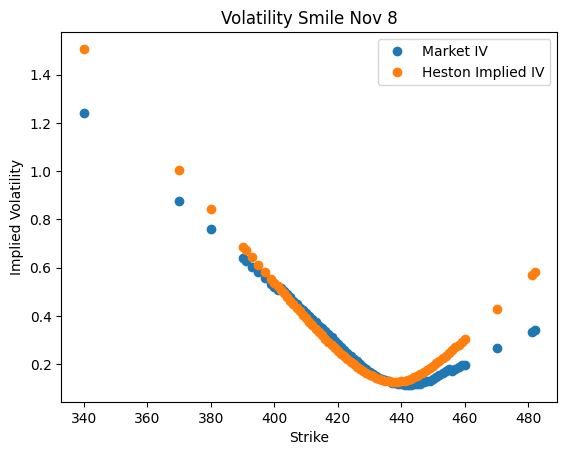
\includegraphics[scale=0.5]{fig/img/option_pricing/heston_smileNov8.png}
    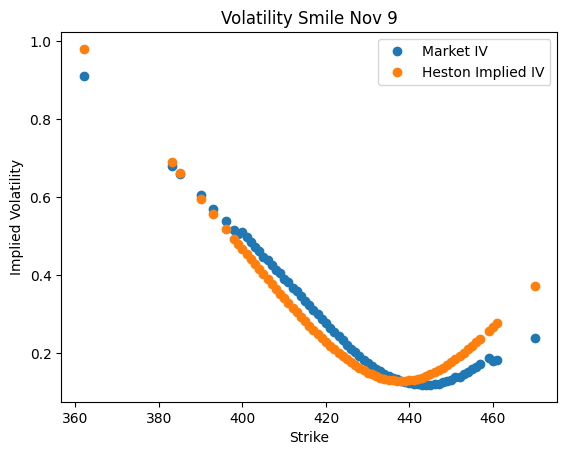
\includegraphics[scale=0.5]{fig/img/option_pricing/hestonSmileNov9.png}
    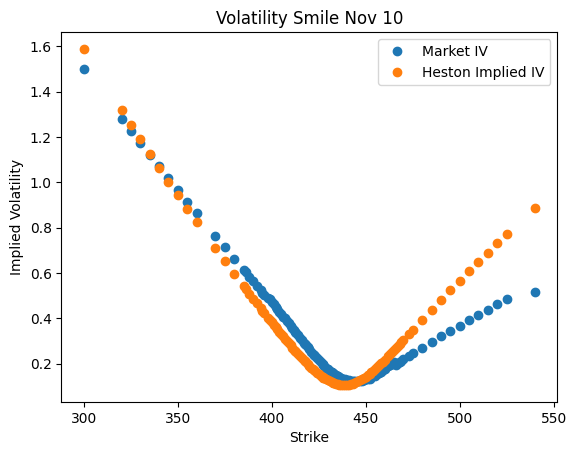
\includegraphics[scale=0.5]{fig/img/option_pricing/hestonSmileNov10.png}
    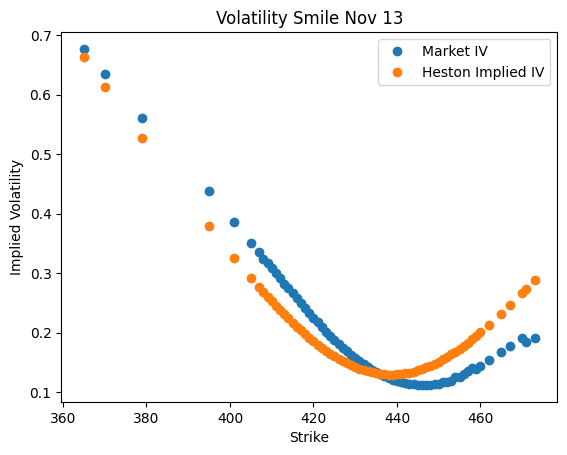
\includegraphics[scale=0.5]{fig/img/option_pricing/hestonSmileNov13.png}
    %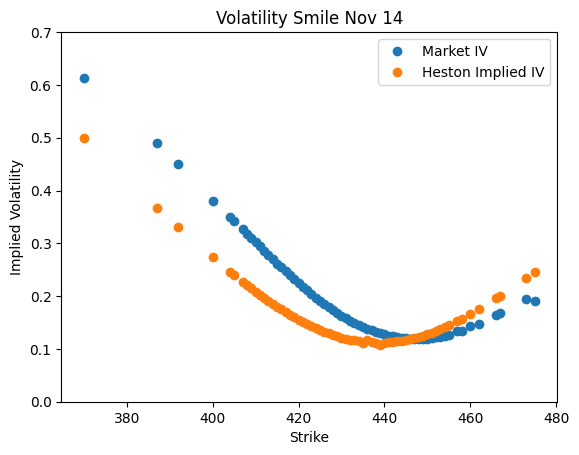
\includegraphics[scale=0.5]{fig/img/option_pricing/hestonSmileNov14.png}
    \caption{Caption}
    \label{fig:enter-label}
\end{figure}